\subsection{Gaussian processes}
\label{sec:chol}

It is common in many uncertainty quantification applications to replace an
expensive model, possibly a discretised partial differential equation with a
cheap surrogate.  This is done so that during a Markov chain Monte Carlo
procedure, likelihood evaluations are cheap.  There are a plethora of different
surrogate choices and strategies for choosing which is appropriate for a
particular application.  Gaussian processes are a common choice, and we explore
their scaling on the KNL architecture here.\todo{citations motherclucker, do you have them?}

Gaussian processes are a probabilistic model for generating random fields
characterised by a mean $\mu$ function and a covariance function $c$.
\begin{equation}
  f(x) \sim \mathcal{N}(\mu(x), c(x, x'))
\end{equation}

They have the property that evaluation of the field at some finite set of
points $(x_1, \ldots, x_n)$ yields a multivariate normal vector with a known
mean vector and symmetric and positive-definite covariance matrix
\begin{equation}
  \begin{pmatrix}
    f(x_1) \\
    \hdots \\
    f(x_n)
  \end{pmatrix}
  \sim \mathcal{N}(\mu, \Sigma).
\end{equation}
Thus, laying down a grid of points at which we wish to model the field yields
the usual Gaussian probability distribution function we are familiar with,
\begin{equation}
  p(x) \propto |\Sigma|^{-1/2} \exp(-\frac12 x^\top \Sigma^{-1} x).
\end{equation}
Notice that evaluation of this probability density function necessitates a
linear solve $\Sigma u = x$.  Since $\Sigma$ is symmetric and positive-definite
a Cholesky factorisation is required.  Iterative approaches exist too, but we
concentrate on the direct approach here.  It is also worth noting that the
covariance function typically takes an exponential form
\begin{equation}
  c(x, x') = \sigma^2 \exp(-\frac12 \| x - x' \|^2 / l^2)
\end{equation}
and so the resulting covariance matrix
\begin{equation}
  \Sigma_{ij} = c(x_i, x_j)
\end{equation}
is very commonly full and dense.  The covariance function can also contain
unknown parameters that need to be inferred in, for example, a hierarchical
Bayesian setting.  The usual approach is taken for evaluation of the
probability density function
\begin{enumerate}
  \item Compute $L$ such that $\Sigma = LL^\top$.
  \item Solve $\Sigma u = x$ using 1.
  \item Compute the inner-product $x^\top u$.
  \item Divide by the square root of the determinant of $\Sigma$.
  \item Return $p$
  \item Go to 1. for the next state in the Markov chain.
\end{enumerate}

QUESO was used to manage the Gaussian process and Markov chain infrastructure.
The bulk of the computational cost lies inside the likelihood function which
necessitates the evaluation of the Gaussian probability density function.
Extensive use of Intel's MKL was used for both the Cholesky factorisation,
subsequent linear solve, and determinant calculation.

Figure~\ref{fig:gp} shows timings of a Gaussian process likelihood evaluation
as a function of number of OpenMP threads.\todo{NM- can you repeat study with MPI? DM- As far as I'm aware, MKL doesn't take an MPI communicator.  MKL is how we do the Cholesky for the GP.}
%NM: can you do the same study with a single OMP thread and vary MPI_tasks? numerous authors have found this to be faster, would be interesting to corroborate
%DM: As far as I'm aware, MKL doesn't take an MPI communicator.  MKL is how we do the Cholesky for the GP.

%
% I would also add a discussion of the timings here. Can you say something about strong-weak scaling?
% this looks like a strong scaling analysis, can you detail more on the speedup?
% also, I can't read those plot axes
%
% DM: I'll update the plot axes.
%
\begin{figure}
  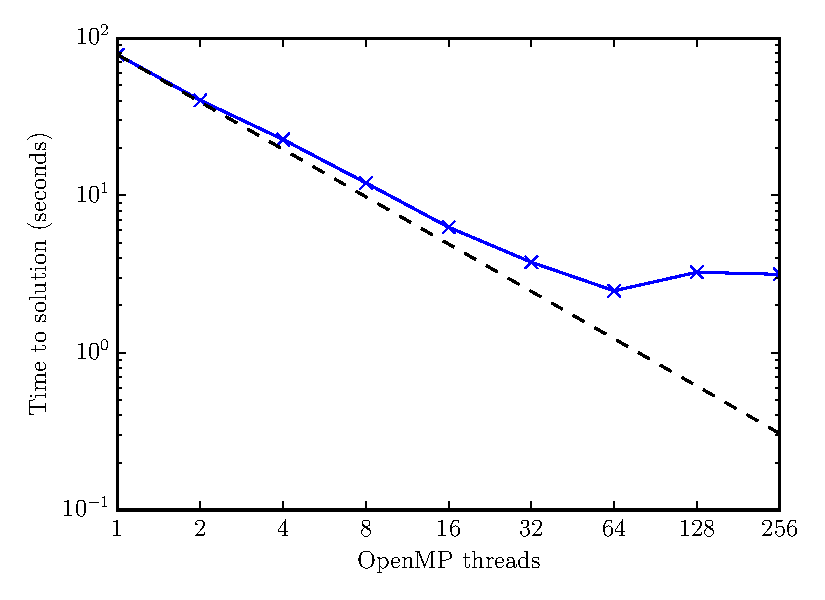
\includegraphics[width=0.45\textwidth]{openmp_scaling_1.pdf}
  \label{fig:gp}
\end{figure}
